\chapter{Arbetet}
\label{sec:arbetet}
Arbetet kan del


Stort problem är att json och json scheman inte skiljer på heltal och reela tal, medan många språk gör det. Specifikt Delphi som systemet utvecklades i.

\section{Systemet i helhet}

När användargränssnittet ska visas första gången, eller efter att en användare valt att trycka på "spara-knappen" (se figur \ref{label}), skickar servern två dokument till klienten. Det dataflödet illustreras i figur \ref{fig:system:ner}. Det ena dokumentet är ett JSON Schema som beskriver vilken data användaren med hjälp av klienten ska kunna se och redigera. Det andra dokumentet som skickas till klienten är den faktiska data som är sparad på servern. Först så parsas schemat och representeras i instanser av \textit{records} eller objekt i Delphi. Sedan används datan för att populera objekten med de korrekta värdena, för att tillsammans skapa modellen. Det sista steget är att det grafiska användargränssnittet genereras och presenteras för användaren.

Varje gång användaren interagerar med användargränssnittet och matar in giltig data, uppdateras modellen vilket i sin tur uppdaterar det grafiska användargränssnittet. Det dataflödet illustreras i figur \ref{fig:system:upp} Detta sker utan någon kontakt med servern. Om användaren är nöjd med sina ändringar och vill spara dem på servern kan användaren trycka på "spara-knappen" (se figur \ref{label}) så uppdateras dataobjektet med de nya värdena från datamodellen, vilket sedan skickas till servern. Efter det börjar systemet igång från början igen.

\begin{figure}
	\begin{subfigure}{0.5\textwidth}
		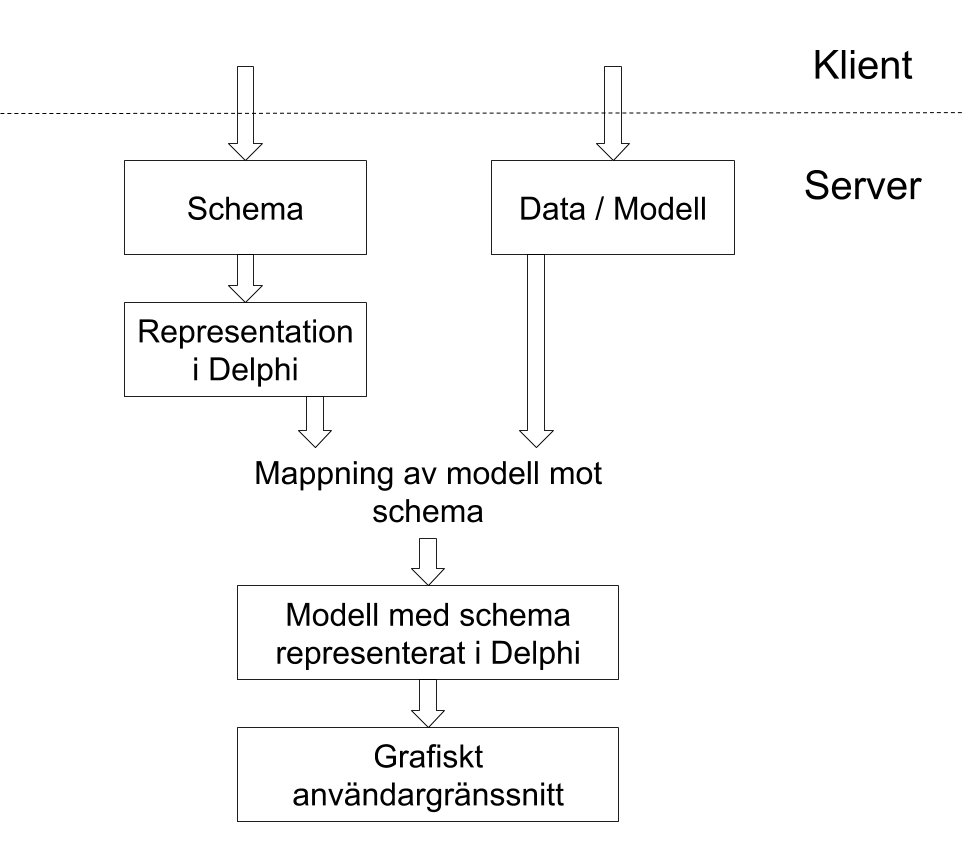
\includegraphics[width=0.9\textwidth,left]{./images/system-ner.png}
		\caption{Flödesschema över systemet}
		\label{fig:system:ner}
	\end{subfigure}
	\begin{subfigure}{0.5\textwidth}
		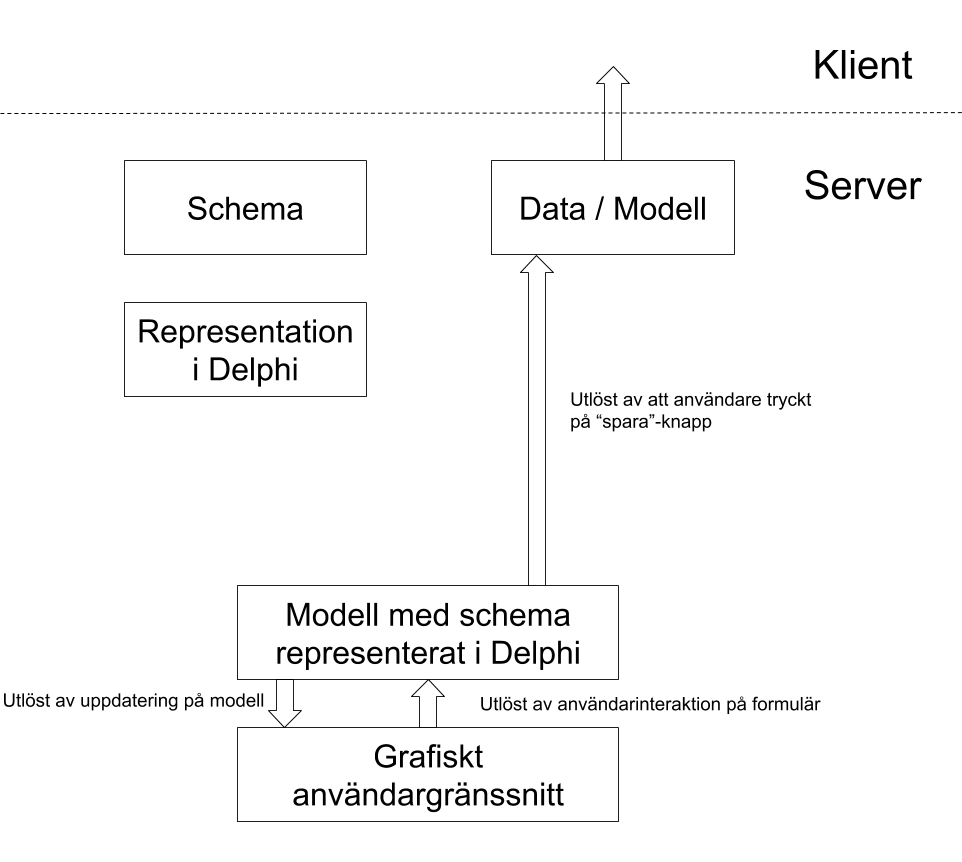
\includegraphics[width=0.9\textwidth,right]{./images/system-upp.png}
		\caption{Flödesschema över systemet}
		\label{fig:system:upp}	
	\end{subfigure}
	\caption{Illustration av dataflöde till och från användargränssnittet}
	\label{fig:system}
\end{figure}

\section{Generering av JSON Schema i Delphi}

Hur JSON Schemat genereras, påverkar inte slutanvändaren, men det påverkar utvecklarna som ska jobba med systemet, och kan hindra vilken funktionalitet som finns tillgänglig i systemet. Ett alternativ är självklart att skriva scheman för hand, men då olika klienter måste ha olika scheman, måste utvecklare se till att rätt schema hamnar på rätt klient vid instalationen av Mimer SoftRadio. Om en kund skulle vilja uppgradera funktionaliteten hos sin installation av Mimer SoftRadio, och därmed behöva tillgång till fler konfigurerbara inställningar i systemet, skulle schemat behöva uppdateras efteråt.

Ett annat alternativ är att basera schemat på inbyggda datatyper i det statiskt typade språket Delphi. Json.NET Schema, NJsonSchema for .NET, typescript-json-schema samt Typson erbjuder exakt den här funktionaliteten i språken .NET respektive TypeScript. För att lägga till extra beskrivningar av datan som språket inte räcker till för, använder .NET-implementationerna \textit{Data Annotation Attributes}, och TypeScript-implementationerna använder experimentella \textit{Decorators}. \cite{Suter,Newtonsoft,El-Dardiry,Bovet} Delphi erbjuder liknande funktionalitet med \textit{Attributes (RTTI)} \cite{Embarcadero2016}. Att annotera datastrukturerna som faktiskt sedan kommer användas i ett system kan automatisera väldigt mycket. Det passar jättebra om det handlar om att bygga ett API där JSON Scheman ska användas för att beskriva för klienter hur och vilken data de kan manipulera. Då kan scheman dynamiskt skapas vid exekvering och de är alltid synkroniserade med datan som systemet är konstruerat för att hantera. Problemet med den lösningen är att schemat i det här arbetet inte ska användas för att beskriva vilken data som kan manipuleras på servern, utan det ska användas för att beskriva hur ett användargränsnitt ska se ut. Den data som ska presenteras på användargränsnittet är en delmängd av all tillgänglig data på servern. Det skulle kunna gå att lägga till annoteringar som beskriver vilken data som ska finnas med på schemat, men det finns enklare lösningar.

Alternativet att handskriva JSON Scheman kräver mycket uppräthållning av scheman och är väldigt mottagligt för misstag hos utvecklarna. Det kräver dock inget system för att dynamiskt generera scheman vid exekvering, då de redan skulle vara genererade. Alternativet att konstruera ett system som använder run-time type information \textit{(RTTI)} är väldigt smidigt för utvecklare under exekvering men kräver relativt mycket utveckling. Ett mellanting skulle vara felsäkert som handskrivna JSON Scheman, men samtidigt dynamiskt genererat vid exekvering för felfria scheman.

JSL är ett exempel på en implementation som erbjuder specifika komplexa datatyper som underlättar genererandet av JSON Scheman. JSL skiljer på datastrukturerna som används för att representera och manipulera data, och själva schemat som används för att beskriva de tidigare nämnda datastrukturerna. \cite{Romanovich} Det ansågs vara ett väldigt praktiskt mellanting. Scheman skrivs för hand men de skrivs inte som JSON Scheman. Istället skrivs de som instanser av komplexa datatyper i Delphi, som sedan under exekvering dynamiskt tolkas för att generera ett JSON Schema. Det här tillåter servern att under exekvering utföra logiska bedömningar för att inkludera exakt det som ska inkluderas i schemat, beroende på vilken version av Mimer SoftRadio operatörsdatorn har, och med vilken tillgänglig funktionalitet datorn har. Schemagenerering är frikopplat från databehandling, men är samtidigt dynamiskt genererat utifrån tillgänglig funktionalitet på operatörsdatorn. Ett exempel på ett genererat schema presenteras i figur \ref{fig:real-schema}.

\begin{figure}
	\inputminted[tabsize=2, frame=single, fontsize=\tiny, framesep=2mm, breaklines]{json}{code/schema.json}
	\vspace{-1.7em}
	\caption{Exempel på genererat schema}
	\label{fig:real-schema}
\end{figure}

Att generera scheman från JSON-filer ansågs inte vara praktiskt genomförbart (se kapitel \ref{sec:forarbete:json-till-schema}), och skulle inte kunna uppräthålla kraven på systemet. Det skulle dessutom helt ta bort möjligheten för utvecklare att beskriva användargränssnittet.

\section{Parsningen av JSON Schema i Delphi}
\label{sec:arbetet:parsning}

Parsningen av JSON Scheman skedde på ett liknande sett som scheman genererades. För att förenkla arbetet skapades en hjälpklass för att hantera scheman i Delphi. Det innehöll olika objekt \textit{(records)} för att representera olika komponenter i JSON Scheman, samt hjälpfunktioner för att generera JSON Scheman utifrån objekten, och parsa JSON Scheman för att sedan få dessa objekt. Ett tillägg till enkla JSON Scheman var att dessa objekt också kunde innehålla värdet av komponenten den innehöll. Utöver hjälpfunktioner för att parsa och generera scheman fanns bland annat också hjälpfunktioner som användes för att bestämma vilken grafisk komponent som skulle användas för att representera datan.

Strukturen av dessa JSON Scheman kunde antas ha en förutsatt struktur, då användningsområdet var väl känt, samt att både klient och server utvecklades med åtanke till varandra och ingen annan tjänst. Alla inställningsfiler som skulle manipuleras av användargränssnittet hade en liknande struktur som figur \ref{fig:profile-file}. Hela filen är ett objekt, med inställningsgrupper som properties. Figuren har bara en inställningsgrupp men det finns möjlighet för fler. Varje inställningsgrupp är också ett objekt, och den har properties som representerar inställningar. Dessa inställningar är alltid en textsträng, ett heltal, eller ett booleskt värde. Det går därför att utforma parsningen utifrån den här förutbestämda strukturen.

\begin{figure}
	\inputminted[tabsize=2, frame=single, fontsize=\small, framesep=2mm, breaklines]{json}{code/0.json}
	\vspace{-1.7em}
	\caption{Exempel på genererat inställningsfil}
	\label{fig:profile-file}
\end{figure}
\FloatBarrier

\noindent
För att både generering och parsning hanterades av samma tjänst ansågs nyckelordet \textit{definitions} och \textit{\$ref} vara onödigt. Parsern hade därför inte stöd för de två nyckelorden. Det var också känt att parsern aldrig skulle behöva hantera vektorer \textit{(array)} som datatyp vilket innebar att alla nyckelord relaterade till array kunde ignoreras i implementationen. Utöver det var den grundläggande strukturen väl känd och därför behövdes inte nyckelord som:

\begin{itemize}
	\item if
	\item then
	\item else
	\item allOf
	\item anyOf
	\item oneOf
	\item not
\end{itemize}

\noindent
Det fanns fler nyckelord som inte implementerades då bara en delmängd av JSON Schema. För att flersvarsalternativ skulle kunna erbjudas i användargränssnittet implementerades stöd för nyckelordet \textit{enum}, dock med vissa tillägg vilket diskuteras mer i kapitel \ref{sec:arbetet:gui}.

Figur \ref{fig:system:ner} beskriver systemet i helhet och där är parsningen en viktig del av dataflödet. Först parsas schemat för att skapa en representation av schemat i Delphi, med de tidigare nämnda objekten. Objekten innehåller också värdet av datan de beskriver men i det första steget är alla värden tomma. Nästa steg är att traversera JSON-filen som innehåller den riktiga datan, och sedan populera objekten med korrekta värden. Först då kan användargränssnittet genereras.

\section{Representation av data i användargänssnittet}
\label{sec:arbetet:gui}

Många implementationer diskuterade i \ref{sec:forarbete:gui-generering} använder ett extra JSON-dokument för att beskriva hur schemat, och modellen schemat representerar ska presenteras i användargränssnittet. Det ansågs vara överflödigt att behöva skicka två dokument som båda ska användas vid exakt samma steg i systemet. Det andra alternativet för att utöka funktionalitet hos JSON Schema är att använda egna nyckelord i schemat som inte finns standardiserade i JSON Schema specifikationerna. Det här arbetet krävde nästan ingen utökad funktionalitet hos JSON Scheman, förutom förbättrad funktionalitet hos \textit{enum} vilket diskuteras mer i kapitel \ref{sec:arbetet:gui:enum}. Det gick att generalisera användargränssnittet tillräckligt för att hantera alla datatyper som systemet använder sig av, och presentera ett relevant användargränssnitt av dem. Nyckelordet \textit{format} kunde erbjuda väldigt hög kontroll av användargränssnittet.

\subsection{Det generella användargränssnittet}

Det enklaste valet av gränssnitt skulle vara att erbjuda en generell JSON editor. Det finns många exempel på användargränssnitt som erbjuder ett grundläggande gränssnitt för att redigera generell JSON-data. De skiljer sig inte mycket mot att skriva JSON manuellt, men kan erbjuda enkel hjälp med nyckelord och formatering. Figur \ref{fig:json-editor} visar JSON Editor Online, vilket är ett exempel på ett sådant användargränssnitt \cite{DeJong2018}. Det skulle behöva begränsa vad användaren skulle kunna mata in med hjälp av JSON Schemat men ett sådant formulär har möjlighet att hantera JSON Data som följer all möjlig sorts struktur. Det vore en stor fördel att kunna erbjuda ett formulär som kan hantera alla möjliga sorters scheman. En nackdel med att använda ett sådant användargränssnitt är att det inte är särskillt anpassat för ändamålet, och gränssnittet blir inte särskillt frikopplat mot datan som ska manipuleras. Det blir dessutom svårt att presentera information till användaren som kan hjälpa användaren förstå hur datan kommer användas.

Ett annat alternativ är att göra som React JSON Schema Form (se figur \ref{fig:react-jsonschema-form}). React JSON Schema Form genererar ett webbformulär utifrån ett JSON Schema och ett extra JSON-dokument som kallas UISchema. \cite{MozillaServices} Användargränssnittet blir mycket mer anpassat till syftet, och lättare att använda. Dessutom utnyttjas annoteringsnyckelorden \textit{title} och \textit{description} från JSON Schemat, för att förklara för användaren vad datan betyder. Det som kan bli svårt med en design som är anpassad efter syftet som ett formulär är hur komplexa JSON-strukturer ska hanteras. Hur skulle exempelvis en vektor innehållande objekt med två properties, varav ena propertyn är ett objekt med två olika vektorer, presenteras på ett användarvänligt sätt? Att även presentera annoteringar som \textit{title} och \textit{description} till alla datanoder i det formuläret vore ännu en till utmaning. En vanlig JSON-Editor klarar av att presentera djupt komplexa datatyper, medan det kan vara väldigt svårt att göra samma sak på ett generellt sätt med formulär. Många lösningar som React JSON Schema Form erbjuder generella formulär som klarar av alla JSON Scheman, med alternativet att specificera mer hur formuläret ska se ut, med hjälp av ett extra JSON-dokument. \cite{MozillaServices} Det är en riktigt bra kompromiss om lösningen måste kunna klara av att presentera djupt komplexa datatyper, som inte följer en förutbestämd struktur.

\begin{figure}
	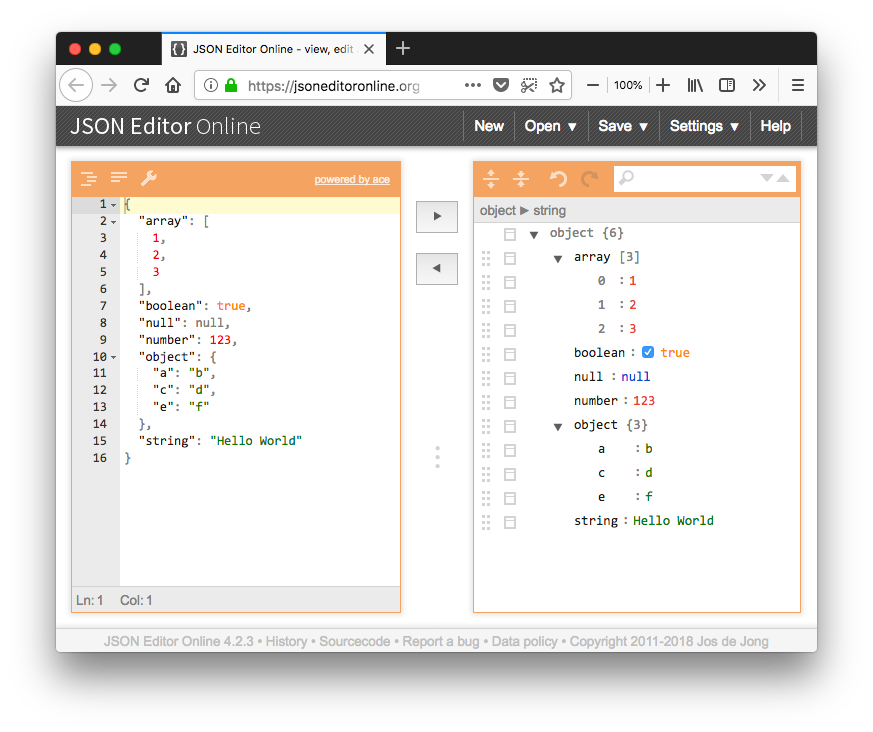
\includegraphics[width=\textwidth]{./images/screenshot-json-editor.png}
	\vspace{-1.7em}
	\caption{JSON Editor Online \cite{DeJong2018}}
	\label{fig:json-editor}
\end{figure}

Datan som skulle presenteras på användargränssnittet i arbetet var varken komplex eller totalt generell. Datan bestod av ett objekt med flera objekt som properties, där de objekten i sin tur var antingen en textsträng, ett heltal eller ett booleskt värde. Datan var som mest tre lager djup. Det gick dessutom att dela in datanoderna i inställningsgrupper och inställningsnoder. Därför kunde både en JSON-editor användas, eller ett formulär. Datan som skulle presenteras ansågs av LSE vara för komplex för många användare att förstå utan en ordentlig förklaring av varje inställningsnod. Därför ansågs ett formulär vara det bästa användargränssnittet. Användargränssnittet presenteras i figur \ref{fig:gui:helhet}. Då användargränssnittet skulle användas både för data med delvis förutbestämd struktur och inte djupt komplex data ansågs ett extra JSON-dokument för att lägga till extra specificering av användargränsnittet överflödigt och onödigt komplext.

\begin{figure}
	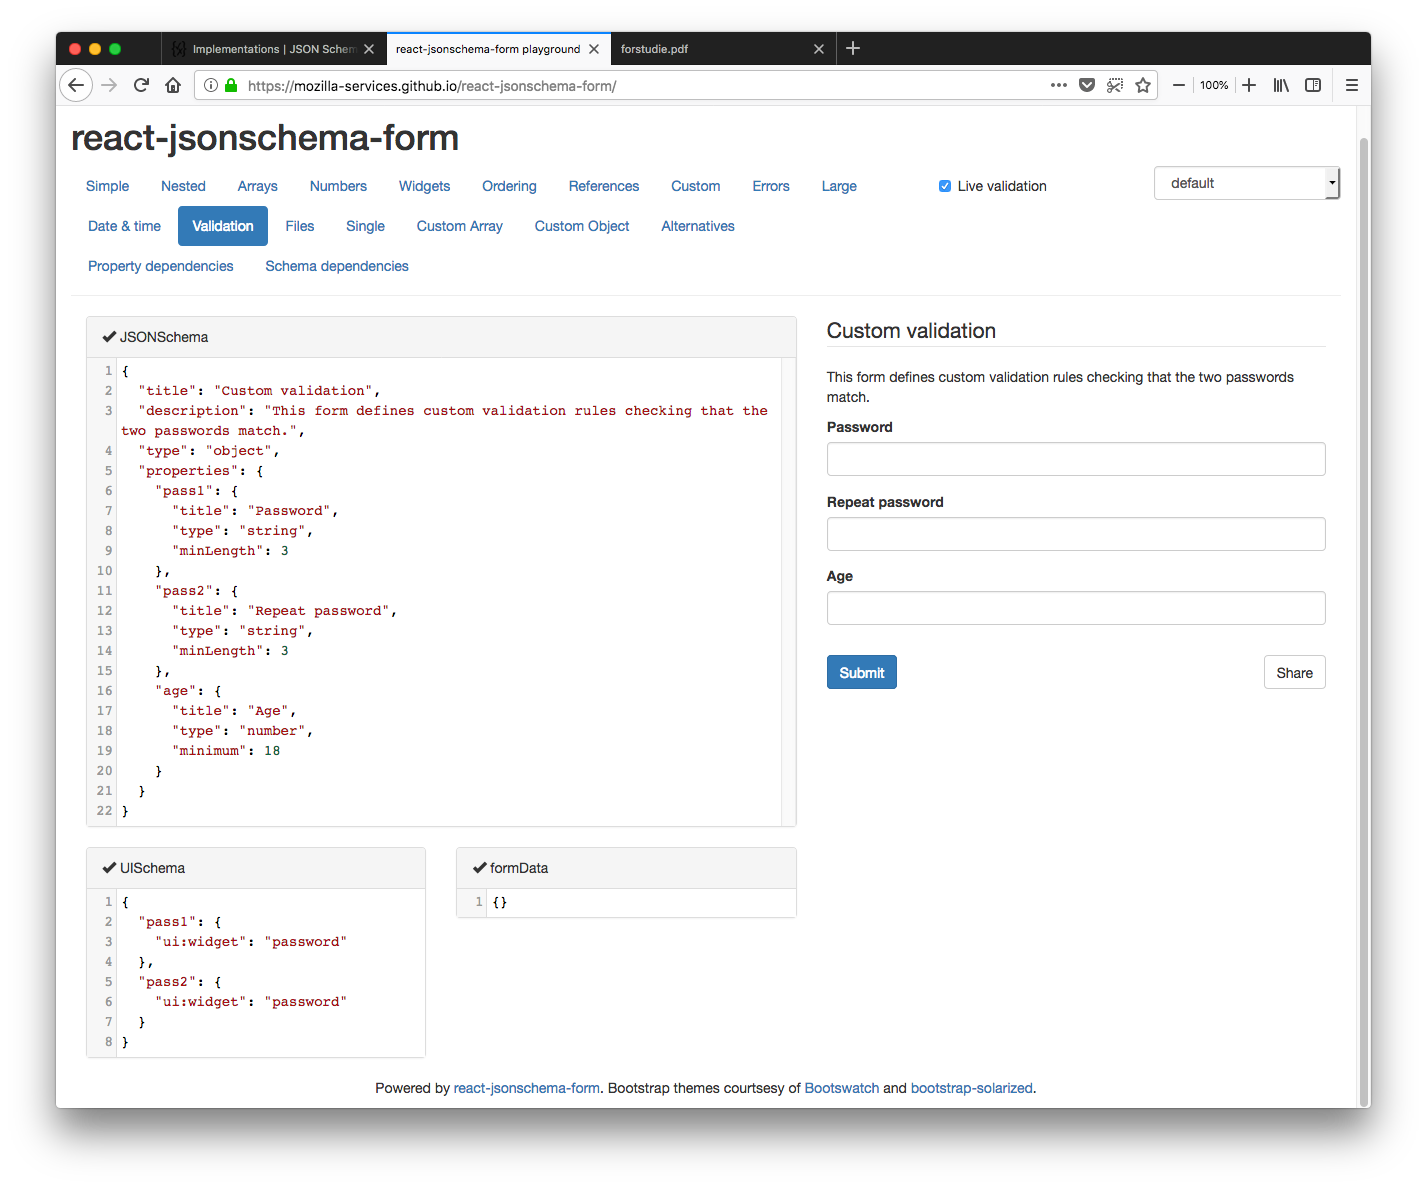
\includegraphics[width=\textwidth]{./images/screenshot-react-jsonschema-form.png}
	\vspace{-1.7em}
	\caption{React JSON Schema Form \cite{MozillaServices}}
	\label{fig:react-jsonschema-form}
\end{figure}

\begin{figure}
	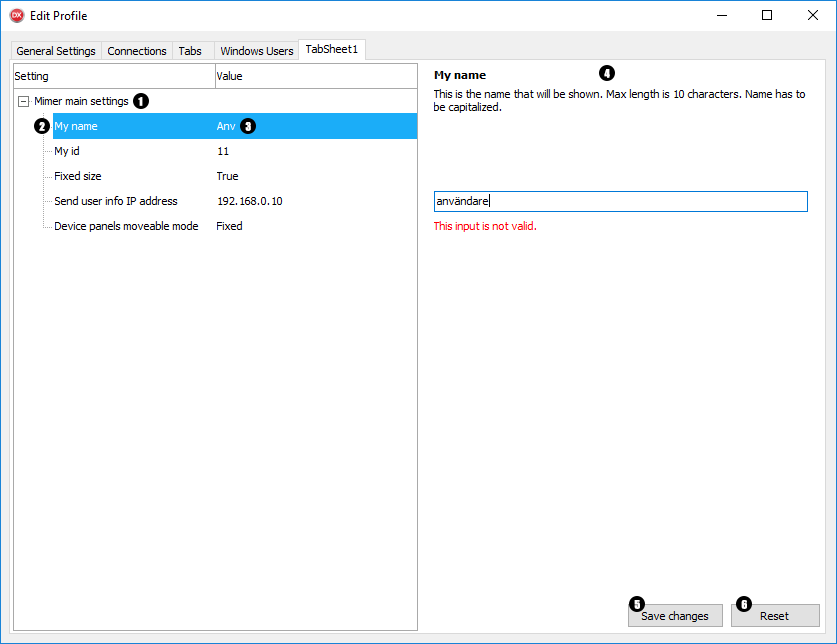
\includegraphics[width=\textwidth]{./images/gui/helhet-copy.png}
	\vspace{-1.7em}
	\caption{Användargränssnittet av administratörsprogrammet \textbf{(TODO! ta ny bild!!!)}}
	\label{fig:gui:helhet}
	\begin{enumerate}
		\item Inställningsgrupp
		\item Namn på inställning
		\item Värde på inställning
		\item Formulär för att ställa in inställning
		\item Spara-knapp
		\item Omstarts-knapp
	\end{enumerate}
\end{figure}

Användargränssnittet som utvecklades blev tvådelat, där ena halvan av gränssnittet användes för att presentera tillgängliga inställningar och inställningsgrupper, samt låta användaren välja en inställning att manipulera. Andra halvan av användargränssnittet användes för att presentera en inställning, med beskrivning av inställningen samt möjligheter att ändra värdet på den valda inställningen. Beslutet grundades på att det skulle vara enkelt för användaren att få en överblick över vilka inställningar som fanns tillgängliga, samtidigt som varje inställning skulle vara enkel att förstå och ändra. Värdena på inställningarna kan alltid synas utan att en inställning väljs men en inställning måste väljas för att kunna bli manipulerad. Namnet på inställningsgrupperna och inställningarna är frikopplade från deras riktiga namn data-filerna och modellen med hjälp av nyckelordet \textit{title} i JSON Schemat.

För att förenkla för användaren erbjuds en omstarts-knapp som raderar alla osparade ändringar och startar om formuläret så att formuläret motsvarar inställningarna på servern. Vid varje användarinteraktion, där en användare manipulerar ett värde på formuläret, propageras ändringen till datamodellen vilket i sin tur uppdaterar hela användargränsnittet, men ändringen skickas inte till servern. Användaren har erbjudits en spara-knapp och först då förmedlas alla ändringar till servern.

\subsection{Hur formuläret förhindrar fel}

Syftet med JSON-scheman är till stor del att förhindra att inkompatibel data sparas och används i applikationer. Det kan handla om att ett användargränssnitt inte är byggt för att presentera viss sorts data, eller att ett helt system upphör att fungera för att systemet inte kunde hantera den sparade datan. Användningen av JSON Scheman i det här arbetet handlar också om att säkerställa att enbart kompatibel data skickas mellan klient och server. En kritisk frågeställning vid utvecklandet av ett intuitivt användargränsnitt är hur felaktiga användarinteraktioner ska hanteras i användargränssnittet.

Den enklaste hanteringen av inkompatibel data, är att när en användare har givit inkompatibel data, kan ett generiskt felmeddelande presenteras, samt att användaren förhindras från att spara datan före användaren givit kompatibel data. Det förlitar sig på att varje inställning har en tillräckligt utförlig förklaring för hur datan ska formateras. Ett annat alternativ är att förhindra att användaren kan mata in felaktig data. Det kan exempelvis handla om att användaren bara kan mata in siffror till formuläret, om datan ska formateras som en siffra. Om användaren försöker mata in en bokstav så ignoreras den användarinteraktionen. Det kan kompleteras med förklaringar av korrekt formatering i inställningsbeskrivningen, men att användaren inte ens kan mata in inkompatibel data är väldigt intuitivt. Det perfekta målet vore att när en användare matar in inkompatibel data, ändrar formuläret datan till den närmsta kompatibla datan. Om en användare matar in siffran 300 i ett formulär som bara tillåter siffror upp till siffran 255 så kan formuläret automatiskt ändra värdet till 255. Det kan dock vara svårt att lösa för mer komplexa situationer.

För att erbjuda en grundlägande användbarhet av formuläret presenterades olika sorters inmatningsfält beroende på om typen av inställning var en textsträng, en siffra eller ett booleskt värde. Detta förhindrade att användare kunde mata in data som var av fel typ. Det fanns fler fall där ännu fler olika inmatningsfällt kunde presenteras beroende på mer formateringsinformation av datan. När det gick så skapades formuläret så att den aldrig tillät användaren att mata in inkompatibel data, men i vissa fall visades bara ett felmeddelande. Hur olika formateringar specificerat i schemat uppräthölls beskrivs i resten av kapitlet.

\subsection{Textsträngar och \textit{format} i användargränssnittet}

När en vald inställning ska vara formaterad som en sträng, presenteras ett inmatningsfält för strängar, som i figur \ref{fig:textstrang}. JSON Schema erbjuder tre valideringsnyckelord enbart för textsträngar: \textit{maxLength}, \textit{minLength} samt \textit{pattern}. Nyckelorden \textit{maxLength} och \textit{minLength} används för att bestämma längden av textsträngen. Nyckelordet \textit{pattern} bestämmer att textsträngen måste följa ett mönster, som specificeras som ett regular expression enligt ECMA 262 regular expression dialect \cite{EcmaInternational2017}. Utöver de tre nyckelorden finns det ett fjärde nyckelord som är applicerbart på textsträngar, vilket är \textit{format}. I de senaste JSON Schema specifikationerna är samtliga åtta definerade format enbart applicerbara på textsträngar. Det går att applicera nyckelordet \textit{format} på vilken datatyp som helst, vilket kort kommer diskuteras senare i rapporten. \cite{Andrews}

\begin{figure}
	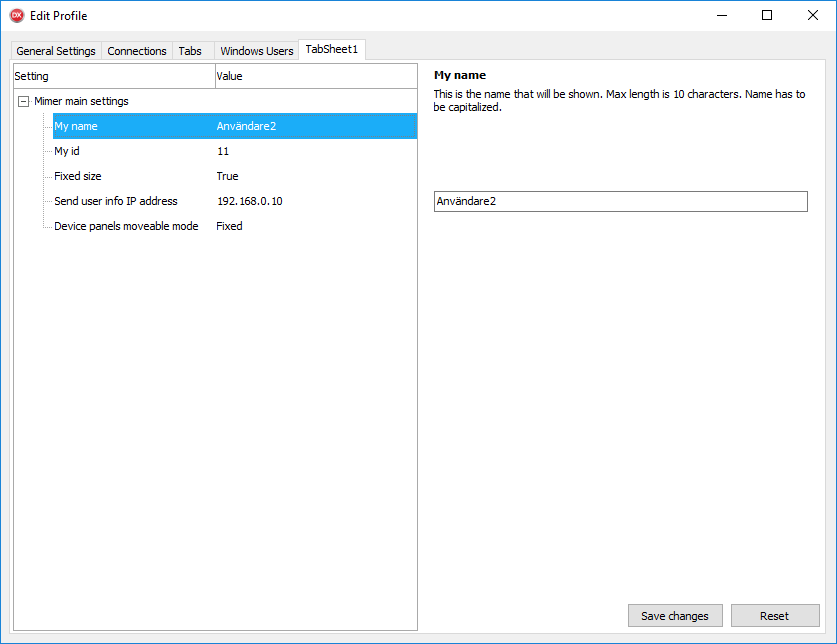
\includegraphics[width=\textwidth]{./images/gui/textstrang.png}
	\vspace{-1.7em}
	\caption{Inmatningsfält för textsträngar}
	\label{fig:textstrang}
\end{figure}

Om en användare försöker mata in en karaktär i inmatningsfältet, och textsträngen redan är lika lång som den maximala tillåtna längden, ignoreras användarinteraktionen. På det sättet går det inte ens för en användare att mata in inkompatibel data, och försöka förstå hur korrekt formaterad data ska se ut. Detta bör kompleteras med en förklaring i beskrivningen av inställningen, så att användaren förstår varför formuläret hanterar användarinteraktioner på det sättet.

Om en användare försöker ta bort så många karraktärer så att textsträngens längd är kortare än den minsta tillåtna längden, presenteras ett felmeddelande och den senaste tillåtna datan sparas i modellen (se figur \ref{fig:textstrang-minLength}). Det skulle kunna gå att förhindra användaren från att ta bort så många karraktärer, men det skulle kunna upplevas som omständigt av användaren, då det kan finnas fall då användaren vill ta bort hela textsträngen för att byta ut textsträngen mot en helt ny. Om användaren skulle förhindras från att ta bort för många karraktärer, och användaren skulle vilja byta ut hela textsträngen mot en helt annan, skulle användaren behöva mata in den nya samtidigt som den gamla delvis var kvar, vilket inte ansågs vara användarvänligt. Att kombinera det med en maximal längd på textsträngar skulle tvinga användaren att hela tiden förhålla sig inom ett intervall av textsträngslängd.

\begin{figure}
	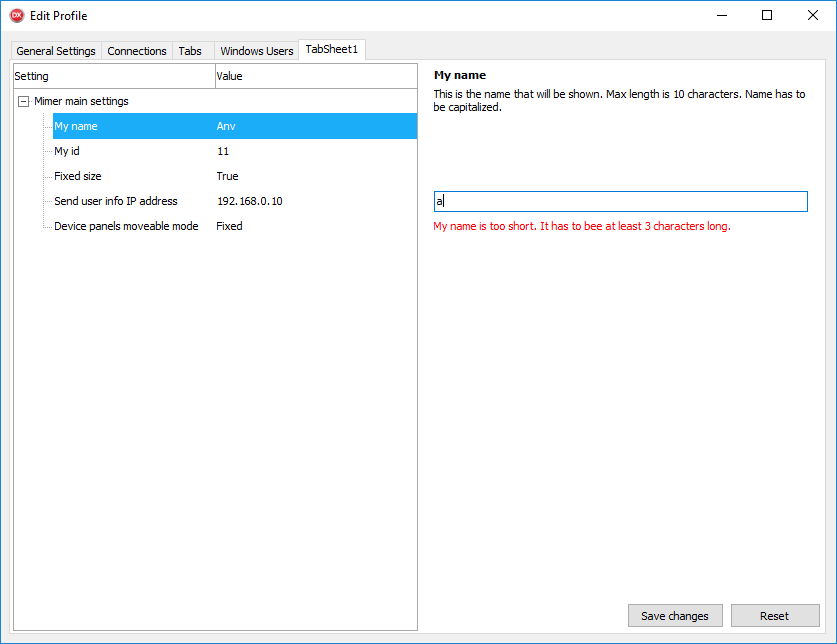
\includegraphics[width=\textwidth]{./images/gui/textstrang-minLength.png}
	\vspace{-1.7em}
	\caption{Felmeddelande vid för kort textsträng}
	\label{fig:textstrang-minLength}
\end{figure}

Om formatet av textsträngen är mer komplext än längd kan \textit{pattern} användas för att specificera väldigt komplexa mönster som en textsträng måste upprätthålla. Det kan exempelvis användas för att specificera att en textsträng ska inledas med versal som i figur \ref{fig:textstrang-pattern}. Då regular expression-mönster kan vara väldigt komplexa och oförutsägbara, är det svårt att hitta ett närmsta kompatiblet värde. Därför presenteras ett felmeddelande när textsträngen inte följer mönstret. Då det inte går att veta hur mönstret fungerar på ett användarvänligt sätt, används ett generiskt felmeddelande, vilket innebär att det är viktigt att inställningsbeskrivningen beskriver formatet som textsträngen ska följa.

\begin{figure}
	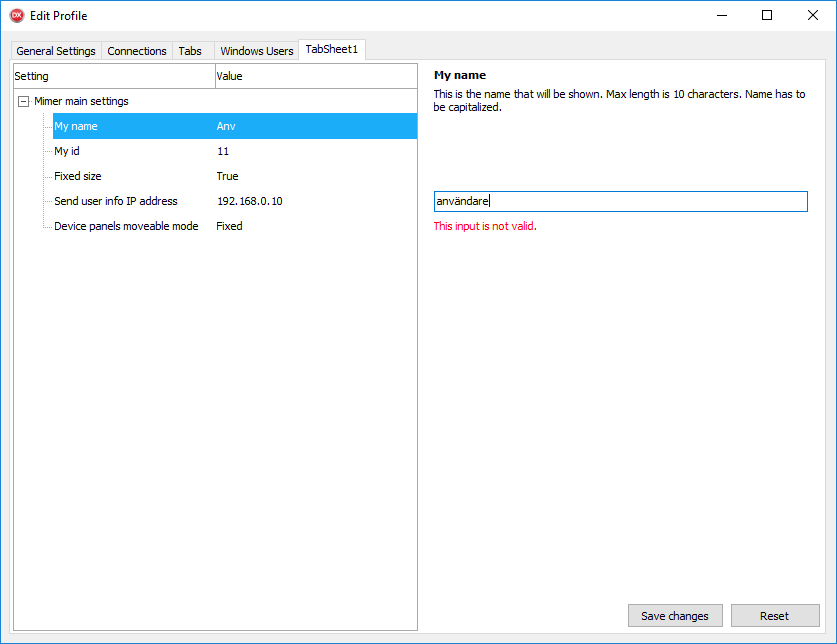
\includegraphics[width=\textwidth]{./images/gui/textstrang-pattern.png}
	\vspace{-1.7em}
	\caption{Felmeddelande vid för textsträng som inte följer regular expression-mönstret}
	\label{fig:textstrang-pattern}
\end{figure}

\FloatBarrier
\subsection{Nyckelordet \textit{format}}

Nyckelordet \textit{pattern} är jättebra för att säkerställa att textsträngar följer ett mer komplext format än enbart längden på textsträngen, men \textit{pattern} kan inte användas för att bestämma hur inmatningsfältet ska se ut. Ibland skulle det passa bättre att presentera ett inmatningsfält som är mer lämpat för en specifik textsträng. Det kan exempelvis passa med ett litet inmatningsfält för korta textsträngar som bara ska vara ett eller några ord, men vid längre texter kanske ett större inmatingsfält behövs. Nyckelordet \textit{format} används både för annotering och validering enligt JSON Schema specifikationerna och får användas för att beskriva egna format på JSON-värden, som inte nödvändigtvis måste följa en standard upprättad av IETF, men som måste vara förutbestämd av alla parter i samma system \cite{Andrews2018}.

För validering kan \textit{format} användas när nyckelordet \textit{pattern} inte räcker, eller blir komplext att använda, och för annotering kan det användas för att förklara formatet av ett JSON-värde. Det kan också användas för att annotera för ett användargränssnitt, att ett JSON-värde borde presenteras på ett specifikt sätt. Figur \ref{fig:textstrang-ip-format} visar hur \textit{format} används för att beskriva att en textsträng ska vara formaterad som en IPv4-adress. I det fallet kan ett specifikt inmatningsfält erbjudas, som bara tillåter användaren att mata in en IPv4-formaterad textsträng.

Nyckelordet \textit{format} kan användas för andra typer än textsträngar och systemet som utvecklas har stöd både på klienten och servern, för att använda \textit{format} till siffror och booleska värden. När \textit{format} används till textsträngar är det viktigt att poängtera att det borde kompleteras med \textit{pattern} om möjligt. Alla delar av systemet ska vara bakåtkompatibla med tidigare versioner av systemet, för en betydligt lång tidsperiod, och om nya sorters \textit{format} läggs till, kan vissa äldre instanser av klienter vara inkompatibla med den sortens \textit{format}.

\begin{figure}
	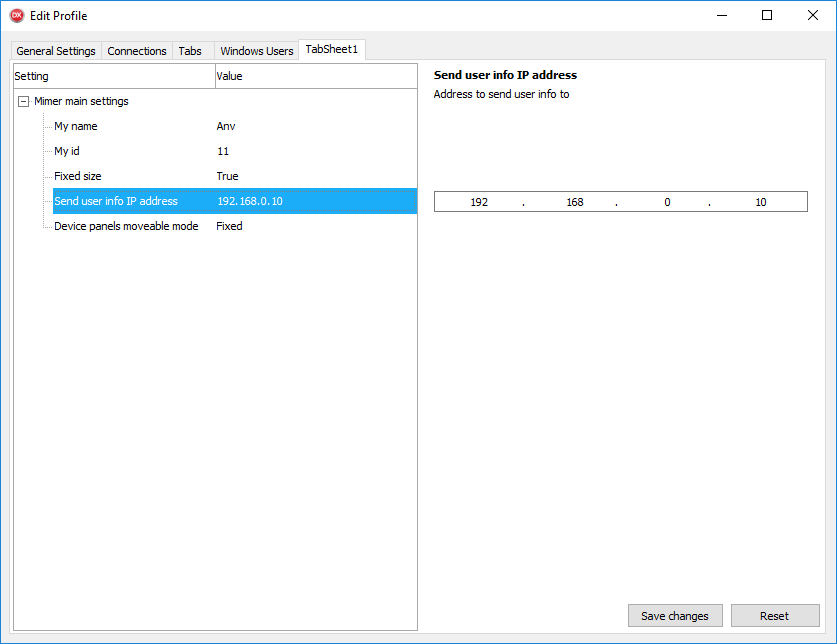
\includegraphics[width=\textwidth]{./images/gui/textstrang-ip.png}
	\vspace{-1.7em}
	\caption{Textsträng formaterad som en IPv4-adress}
	\label{fig:textstrang-ip-format}
\end{figure}


\FloatBarrier
\subsection{Booleska värden och heltal i användargränssnittet}

Booleska värden kan bara vara ett av två värden. Inmatningsfältet som valdes för att presentera booleska värden blev en kryssruta, som visas i figur \ref{fig:bool}. Det finns ingen möjlighet för användaren att mata in ett annat värde än de två tillåtna värdena. Om användargränssnittet ska presentera något annat värde än \textit{true} eller \textit{false} kan nyckelordet \textit{enum} användas, vilket diskuteras mer senare.

\begin{figure}
	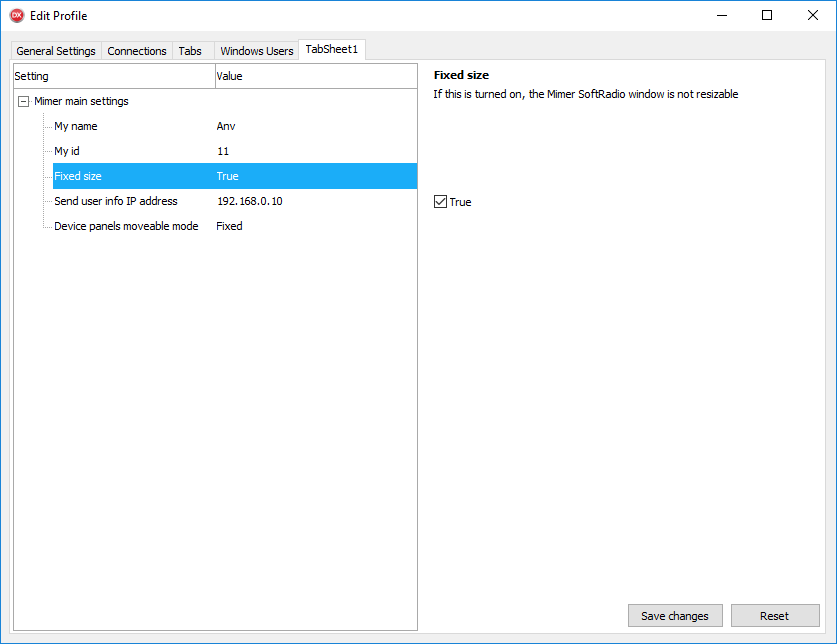
\includegraphics[width=\textwidth]{./images/gui/bool.png}
	\vspace{-1.7em}
	\caption{Kryssruta för ett booleskt värde}
	\label{fig:bool}
\end{figure}

Utöver booleska värden och textsträngar skulle systemet klara av att hantera heltal. Då hanteringen av flyttal fortfarande ansågs vara experimentel och ofärdig, samt att det saknades behov av flyttal så implementerades bara stöd för heltal. Då både klient och server utvecklades med hänsyn till varandra, i samma språk (Delphi), samt att systemet inte var byggt för att hantera flyttal, kunde alla siffror antas vara heltal, och inga oklarheter kring vad som räknas som heltal (se kapitel \ref{sec:teori:schema:float}) behövde hanteras. Om något tal skulle skickas som ett flyttal skulle det talet avrundas och hanteras som ett heltal vid parsningen av JSON-filen.

Heltal presenterades som i figur \ref{fig:heltal}. Inmatningsfältet hanterar endast siffror och har dessutom två hjälpknappar för att höja och sänka värdet i steg. Det finns fem valideringsnyckelord enbart för siffror: \textit{multipleOf}, \textit{maximum}, \textit{exclusiveMaximum}, \textit{minimum} samt \textit{exclusiveMinimum}. Nyckelordet \textit{multipleOf} kräver att siffran som valideras ska vara jämnt delbart med värdet beskrivet av \textit{multipleOf}. Användningsområdet för \textit{multipleOf} ansågs inte vara applicerbart för systemet och därför ignorerades. De resterande fyra nyckelorden specificerar ett interval som siffran måste befinna inom. Om en användare försökte mata in ett värde som var utanför intervallet så ändrades värdet till det närmaste kompatibla värdet inom intervallet. \cite{Andrews2018}

\begin{figure}
	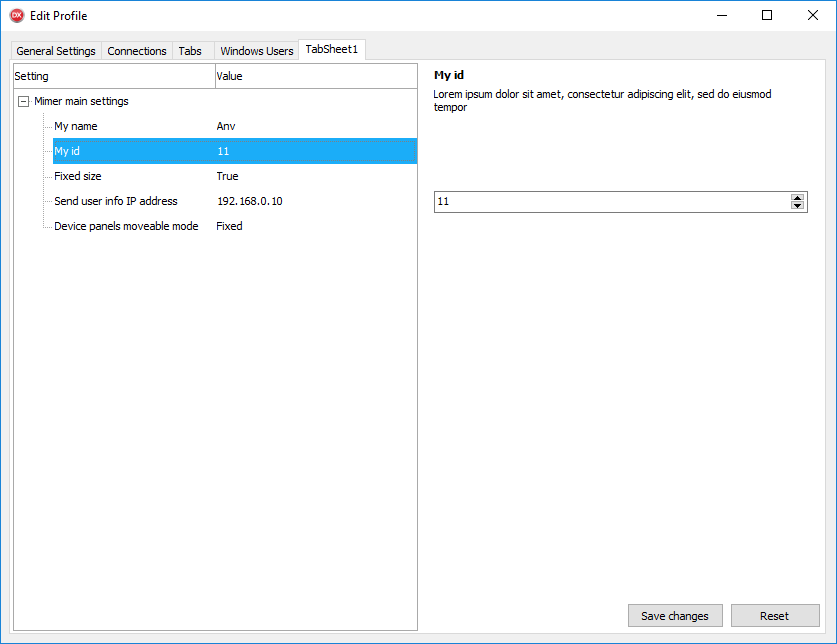
\includegraphics[width=\textwidth]{./images/gui/heltal.png}
	\vspace{-1.7em}
	\caption{Inmatningsfält för heltal}
	\label{fig:heltal}
\end{figure}

Om stöd för flyttal skulle behövas i framtiden, föreslås att nyckelordet \textit{format} används för att specificera det. Det skulle kunna hanteras på ett sätt som är bakåtkompatibelt med klienter som bara kan hantera heltal, genom att de klienterna hanterar flyttalen som heltal, samtidigt som nyare klienter kan hantera flyttalen som flyttal.

\subsection{Flervalsalternativ och \textit{enum} i användargränssnittet}
\label{sec:arbetet:gui:enum}

Vissa inställningar hade så pass begränsade tillåtna alternativ att bara ett fåtal alternativ på värden var tillåtna. Då användes nyckelordet \textit{enum}. Nyckelordet \textit{enum} används för att specificera en lista med tillåtna värden. Inmatningsfältet som valdes var en lista med alternativ som användaren kan välja, som presenteras i figur \ref{fig:enum}. Det fanns aldrig fall då olika alternativ skulle vara av olika typer, trots att JSON Schema tillåter det \cite{Andrews2018}.

\begin{figure}
	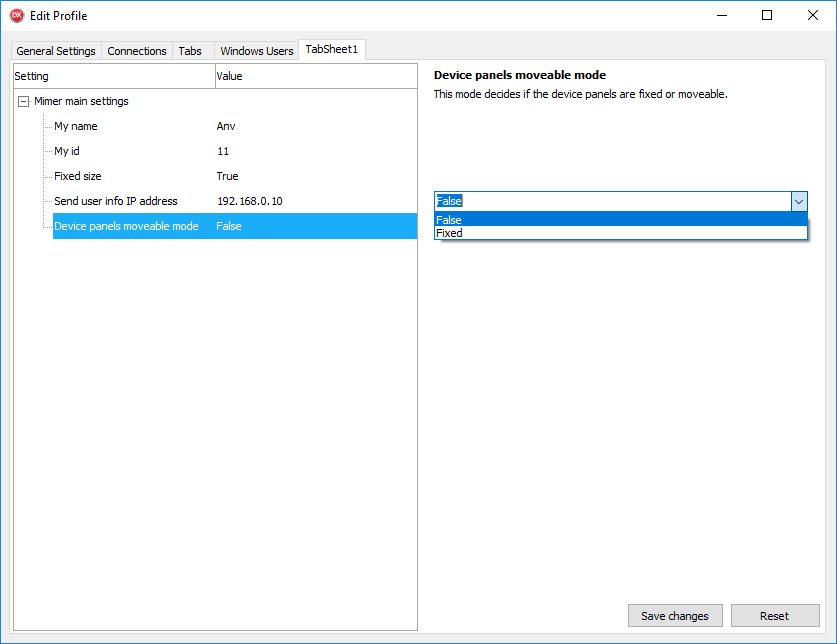
\includegraphics[width=\textwidth]{./images/gui/enum.png}
	\vspace{-1.7em}
	\caption{Inmatningsfält för \textit{enum}}
	\label{fig:enum}
\end{figure}

Enum tillåter inga alternativ för att annotera de förutsatta värdena med metadatainformation som \textit{title} eller \textit{description}. Det innebär att värdena som \textit{enum} specificerar, inte går att koppla till någon annan representation än det faktiska värdet. Ett problem skulle exempelvis kunna uppstå om ett värde bara få ha värdena \textit{1}, \textit{2} eller \textit{3} i en JSON-fil, men användarna ska presenteras med \textit{one}, \textit{two} och \textit{three} som svarsalternativ. React JSON Schema Form bemöter det problemet med att utöka JSON Schema och lägga till nyckelordet \textit{enumNames} som i figur \ref{fig:enum-example:extra-array} \cite{MozillaServices}. Användandet av det nyckelordet är inkompatibelt med JSON Schema \cite{Andrews2018}. Dessutom finns det massor av oklarheter över hur fall skulle hanteras om \textit{enumNames} finns men \textit{enum} saknas, eller om \textit{enumNames} och \textit{enum} innehåller olika antal element.

\begin{figure}
	\inputminted[tabsize=2, frame=single, fontsize=\small, framesep=2mm, breaklines]{json}{code/enum-example/extra-array.json}
	\vspace{-1.7em}
	\caption{Hur React JSON Schema Form föreslår \textit{enumNames} \cite{MozillaServices}}
	\label{fig:enum-example:extra-array}
\end{figure}

Ett annat förslag som React JSON Schema Form föreslår är användandet av nyckelordet \textit{anyOf}, vilket är helt kompatibelt med JSON Schema specifikationerna men är väldigt verbost och använder \textit{anyOf} på ett sätt som det inte ursprungligen är menat för att användas på \cite{MozillaServices, Andrews2018}. Dessutom kräver deras implementation att nyckelordet \textit{enum} ska användas för att definera listor innehållande ett konstant värde, vilket inte är syftet med \textit{enum} \cite{Andrews2018}. Deras förslag visas i figur \ref{fig:enum-example:any-of}. Jag föreslår användandet av nyckelordet \textit{const} istället, vilket visas i figur \ref{fig:enum-example:any-of-const}. Nyckelordet är till för att specificera att en definition bara får ha ett enda konstant värde och är mindre än ett år gammalt, vilket kan vara en anledning till att React JSON Schema Form inte användt \textit{const} i sin implementation \cite{Andrews2018}.

\begin{figure}
	\begin{subfigure}[t]{0.47\textwidth}
		\inputminted[tabsize=2, frame=single, fontsize=\small, framesep=2mm, breaklines]{json}{code/enum-example/any-of.json}
		\vspace{-1.2em}
		\caption{React JSON Schema Forms alternativ till \textit{enumNames} \cite{MozillaServices}}
		\label{fig:enum-example:any-of}
	\end{subfigure}\hfill
	\begin{subfigure}[t]{0.47\textwidth}
		\inputminted[tabsize=2, frame=single, fontsize=\small, framesep=2mm, breaklines]{json}{code/enum-example/any-of-const.json}
		\vspace{-1.2em}
		\caption{Ett modernare förslag av React JSON Schema Forms förslag med \textit{const}}
		\label{fig:enum-example:any-of-const}
	\end{subfigure}
	\caption{Olika JSON Schema-kompatibla implementationer på alternativ för \textit{enum}}
	\label{fig:enum-example:any-of-examples}
\end{figure}

Lösningen att använda \textit{anyOf} är helt kompatibelt med JSON Schema men kan introducera många risker för fel, då \textit{anyOf} kan användas för att definera flera olika generella definitioner, vilket är mycket mer komplext än att använda \textit{enum} för förbestämda värden. Jag föreslår ett fjärde alternativ vilket varken introducerar fler nyckelord, eller förlitar sig på att olika nyckelord förhåller sig korrekt till varandra, men som inte är helt kompatibelt med de nuvarande JSON Schema specifikationerna. Jag föreslår att \textit{enum} används som tidigare för att specificera förutbestämda värden, men att ett värde också kan vara ett objekt med vissa bestämda nyckelord som används för annotering. Figur \ref{fig:enum-example:const} är ett exempel på det formatet. Nyckelorden \textit{title}, \textit{description} och \textit{const} skulle kunna reserveras. Ett problem vore hur en parser skulle kunna skilja på ett objekt som faktiskt innehåller en \textit{property} med namnet \textit{title}, men det skulle kunna vara bestämt att om ett element i listan i \textit{enum} innehåller en \textit{const-property} så kommer eventuella \textit{title} och \textit{description} användas som metadata för värdet i \textit{const}. Om ett objekt med en \textit{property} med namnet \textit{title} ska specificeras i \textit{enum} så räcker det med att placera det objektet i ett objekt under dess \textit{const-property} som i figur \ref{fig:enum-example:title}. Självklart går det dessutom att blanda element som bara är värdet de representerar med annoterade objekt. Arbetet använde den här metoden för att hantera \textit{enums} och flervalsalternativ.

\begin{figure}
	\begin{subfigure}[t]{0.47\textwidth}
		\inputminted[tabsize=2, frame=single, fontsize=\small, framesep=2mm, breaklines]{json}{code/enum-example/const.json}
		\vspace{-1.2em}
		\caption{Enkelt förslag på utökning av enum}
		\label{fig:enum-example:const}
	\end{subfigure}\hfill
	\begin{subfigure}[t]{0.47\textwidth}
		\inputminted[tabsize=2, frame=single, fontsize=\small, framesep=2mm, breaklines]{json}{code/enum-example/nested.json}
		\vspace{-1.2em}
		\caption{Förslag på utökning av enum med objekt som använder \textit{title}}
		\label{fig:enum-example:title}
	\end{subfigure}
	\caption{Förslag på utökning av \textit{enums} i JSON Scheman}
\end{figure}